
%% bare_conf.tex
%% V1.3
%% 2007/01/11
%% by Michael Shell
%% See:
%% http://www.michaelshell.org/
%% for current contact information.
%%
%% This is a skeleton file demonstrating the use of IEEEtran.cls
%% (requires IEEEtran.cls version 1.7 or later) with an IEEE conference paper.
%%
%% Support sites:
%% http://www.michaelshell.org/tex/ieeetran/
%% http://www.ctan.org/tex-archive/macros/latex/contrib/IEEEtran/
%% and
%% http://www.ieee.org/

%%*************************************************************************
%% Legal Notice:
%% This code is offered as-is without any warranty either expressed or
%% implied; without even the implied warranty of MERCHANTABILITY or
%% FITNESS FOR A PARTICULAR PURPOSE! 
%% User assumes all risk.
%% In no event shall IEEE or any contributor to this code be liable for
%% any damages or losses, including, but not limited to, incidental,
%% consequential, or any other damages, resulting from the use or misuse
%% of any information contained here.
%%
%% All comments are the opinions of their respective authors and are not
%% necessarily endorsed by the IEEE.
%%
%% This work is distributed under the LaTeX Project Public License (LPPL)
%% ( http://www.latex-project.org/ ) version 1.3, and may be freely used,
%% distributed and modified. A copy of the LPPL, version 1.3, is included
%% in the base LaTeX documentation of all distributions of LaTeX released
%% 2003/12/01 or later.
%% Retain all contribution notices and credits.
%% ** Modified files should be clearly indicated as such, including  **
%% ** renaming them and changing author support contact information. **
%%
%% File list of work: IEEEtran.cls, IEEEtran_HOWTO.pdf, bare_adv.tex,
%%                    bare_conf.tex, bare_jrnl.tex, bare_jrnl_compsoc.tex
%%*************************************************************************

% *** Authors should verify (and, if needed, correct) their LaTeX system  ***
% *** with the testflow diagnostic prior to trusting their LaTeX platform ***
% *** with production work. IEEE's font choices can trigger bugs that do  ***
% *** not appear when using other class files.                            ***
% The testflow support page is at:
% http://www.michaelshell.org/tex/testflow/



% Note that the a4paper option is mainly intended so that authors in
% countries using A4 can easily print to A4 and see how their papers will
% look in print - the typesetting of the document will not typically be
% affected with changes in paper size (but the bottom and side margins will).
% Use the testflow package mentioned above to verify correct handling of
% both paper sizes by the user's LaTeX system.
%
% Also note that the "draftcls" or "draftclsnofoot", not "draft", option
% should be used if it is desired that the figures are to be displayed in
% draft mode.
%
\documentclass[10pt, conference, compsocconf]{IEEEtran}
% Add the compsocconf option for Computer Society conferences.
%
% If IEEEtran.cls has not been installed into the LaTeX system files,
% manually specify the path to it like:
% \documentclass[conference]{../sty/IEEEtran}





% Some very useful LaTeX packages include:
% (uncomment the ones you want to load)


% *** MISC UTILITY PACKAGES ***
%
%\usepackage{ifpdf}
% Heiko Oberdiek's ifpdf.sty is very useful if you need conditional
% compilation based on whether the output is pdf or dvi.
% usage:
% \ifpdf
%   % pdf code
% \else
%   % dvi code
% \fi
% The latest version of ifpdf.sty can be obtained from:
% http://www.ctan.org/tex-archive/macros/latex/contrib/oberdiek/
% Also, note that IEEEtran.cls V1.7 and later provides a builtin
% \ifCLASSINFOpdf conditional that works the same way.
% When switching from latex to pdflatex and vice-versa, the compiler may
% have to be run twice to clear warning/error messages.






% *** CITATION PACKAGES ***
%
%\usepackage{cite}
% cite.sty was written by Donald Arseneau
% V1.6 and later of IEEEtran pre-defines the format of the cite.sty package
% \cite{} output to follow that of IEEE. Loading the cite package will
% result in citation numbers being automatically sorted and properly
% "compressed/ranged". e.g., [1], [9], [2], [7], [5], [6] without using
% cite.sty will become [1], [2], [5]--[7], [9] using cite.sty. cite.sty's
% \cite will automatically add leading space, if needed. Use cite.sty's
% noadjust option (cite.sty V3.8 and later) if you want to turn this off.
% cite.sty is already installed on most LaTeX systems. Be sure and use
% version 4.0 (2003-05-27) and later if using hyperref.sty. cite.sty does
% not currently provide for hyperlinked citations.
% The latest version can be obtained at:
% http://www.ctan.org/tex-archive/macros/latex/contrib/cite/
% The documentation is contained in the cite.sty file itself.






% *** GRAPHICS RELATED PACKAGES ***
%
\ifCLASSINFOpdf
  % \usepackage[pdftex]{graphicx}
  % declare the path(s) where your graphic files are
  % \graphicspath{{../pdf/}{../jpeg/}}
  % and their extensions so you won't have to specify these with
  % every instance of \includegraphics
  % \DeclareGraphicsExtensions{.pdf,.jpeg,.png}
\else
  % or other class option (dvipsone, dvipdf, if not using dvips). graphicx
  % will default to the driver specified in the system graphics.cfg if no
  % driver is specified.
  % \usepackage[dvips]{graphicx}
  % declare the path(s) where your graphic files are
  % \graphicspath{{../eps/}}
  % and their extensions so you won't have to specify these with
  % every instance of \includegraphics
  % \DeclareGraphicsExtensions{.eps}
\fi
% graphicx was written by David Carlisle and Sebastian Rahtz. It is
% required if you want graphics, photos, etc. graphicx.sty is already
% installed on most LaTeX systems. The latest version and documentation can
% be obtained at: 
% http://www.ctan.org/tex-archive/macros/latex/required/graphics/
% Another good source of documentation is "Using Imported Graphics in
% LaTeX2e" by Keith Reckdahl which can be found as epslatex.ps or
% epslatex.pdf at: http://www.ctan.org/tex-archive/info/
%
% latex, and pdflatex in dvi mode, support graphics in encapsulated
% postscript (.eps) format. pdflatex in pdf mode supports graphics
% in .pdf, .jpeg, .png and .mps (metapost) formats. Users should ensure
% that all non-photo figures use a vector format (.eps, .pdf, .mps) and
% not a bitmapped formats (.jpeg, .png). IEEE frowns on bitmapped formats
% which can result in "jaggedy"/blurry rendering of lines and letters as
% well as large increases in file sizes.
%
% You can find documentation about the pdfTeX application at:
% http://www.tug.org/applications/pdftex





% *** MATH PACKAGES ***
%
%\usepackage[cmex10]{amsmath}
% A popular package from the American Mathematical Society that provides
% many useful and powerful commands for dealing with mathematics. If using
% it, be sure to load this package with the cmex10 option to ensure that
% only type 1 fonts will utilized at all point sizes. Without this option,
% it is possible that some math symbols, particularly those within
% footnotes, will be rendered in bitmap form which will result in a
% document that can not be IEEE Xplore compliant!
%
% Also, note that the amsmath package sets \interdisplaylinepenalty to 10000
% thus preventing page breaks from occurring within multiline equations. Use:
%\interdisplaylinepenalty=2500
% after loading amsmath to restore such page breaks as IEEEtran.cls normally
% does. amsmath.sty is already installed on most LaTeX systems. The latest
% version and documentation can be obtained at:
% http://www.ctan.org/tex-archive/macros/latex/required/amslatex/math/





% *** SPECIALIZED LIST PACKAGES ***
%
%\usepackage{algorithmic}
% algorithmic.sty was written by Peter Williams and Rogerio Brito.
% This package provides an algorithmic environment fo describing algorithms.
% You can use the algorithmic environment in-text or within a figure
% environment to provide for a floating algorithm. Do NOT use the algorithm
% floating environment provided by algorithm.sty (by the same authors) or
% algorithm2e.sty (by Christophe Fiorio) as IEEE does not use dedicated
% algorithm float types and packages that provide these will not provide
% correct IEEE style captions. The latest version and documentation of
% algorithmic.sty can be obtained at:
% http://www.ctan.org/tex-archive/macros/latex/contrib/algorithms/
% There is also a support site at:
% http://algorithms.berlios.de/index.html
% Also of interest may be the (relatively newer and more customizable)
% algorithmicx.sty package by Szasz Janos:
% http://www.ctan.org/tex-archive/macros/latex/contrib/algorithmicx/




% *** ALIGNMENT PACKAGES ***
%
%\usepackage{array}
% Frank Mittelbach's and David Carlisle's array.sty patches and improves
% the standard LaTeX2e array and tabular environments to provide better
% appearance and additional user controls. As the default LaTeX2e table
% generation code is lacking to the point of almost being broken with
% respect to the quality of the end results, all users are strongly
% advised to use an enhanced (at the very least that provided by array.sty)
% set of table tools. array.sty is already installed on most systems. The
% latest version and documentation can be obtained at:
% http://www.ctan.org/tex-archive/macros/latex/required/tools/


%\usepackage{mdwmath}
%\usepackage{mdwtab}
% Also highly recommended is Mark Wooding's extremely powerful MDW tools,
% especially mdwmath.sty and mdwtab.sty which are used to format equations
% and tables, respectively. The MDWtools set is already installed on most
% LaTeX systems. The lastest version and documentation is available at:
% http://www.ctan.org/tex-archive/macros/latex/contrib/mdwtools/


% IEEEtran contains the IEEEeqnarray family of commands that can be used to
% generate multiline equations as well as matrices, tables, etc., of high
% quality.


%\usepackage{eqparbox}
% Also of notable interest is Scott Pakin's eqparbox package for creating
% (automatically sized) equal width boxes - aka "natural width parboxes".
% Available at:
% http://www.ctan.org/tex-archive/macros/latex/contrib/eqparbox/





% *** SUBFIGURE PACKAGES ***
%\usepackage[tight,footnotesize]{subfigure}
% subfigure.sty was written by Steven Douglas Cochran. This package makes it
% easy to put subfigures in your figures. e.g., "Figure 1a and 1b". For IEEE
% work, it is a good idea to load it with the tight package option to reduce
% the amount of white space around the subfigures. subfigure.sty is already
% installed on most LaTeX systems. The latest version and documentation can
% be obtained at:
% http://www.ctan.org/tex-archive/obsolete/macros/latex/contrib/subfigure/
% subfigure.sty has been superceeded by subfig.sty.



%\usepackage[caption=false]{caption}
%\usepackage[font=footnotesize]{subfig}
% subfig.sty, also written by Steven Douglas Cochran, is the modern
% replacement for subfigure.sty. However, subfig.sty requires and
% automatically loads Axel Sommerfeldt's caption.sty which will override
% IEEEtran.cls handling of captions and this will result in nonIEEE style
% figure/table captions. To prevent this problem, be sure and preload
% caption.sty with its "caption=false" package option. This is will preserve
% IEEEtran.cls handing of captions. Version 1.3 (2005/06/28) and later 
% (recommended due to many improvements over 1.2) of subfig.sty supports
% the caption=false option directly:
%\usepackage[caption=false,font=footnotesize]{subfig}
%
% The latest version and documentation can be obtained at:
% http://www.ctan.org/tex-archive/macros/latex/contrib/subfig/
% The latest version and documentation of caption.sty can be obtained at:
% http://www.ctan.org/tex-archive/macros/latex/contrib/caption/




% *** FLOAT PACKAGES ***
%
%\usepackage{fixltx2e}
% fixltx2e, the successor to the earlier fix2col.sty, was written by
% Frank Mittelbach and David Carlisle. This package corrects a few problems
% in the LaTeX2e kernel, the most notable of which is that in current
% LaTeX2e releases, the ordering of single and double column floats is not
% guaranteed to be preserved. Thus, an unpatched LaTeX2e can allow a
% single column figure to be placed prior to an earlier double column
% figure. The latest version and documentation can be found at:
% http://www.ctan.org/tex-archive/macros/latex/base/



%\usepackage{stfloats}
% stfloats.sty was written by Sigitas Tolusis. This package gives LaTeX2e
% the ability to do double column floats at the bottom of the page as well
% as the top. (e.g., "\begin{figure*}[!b]" is not normally possible in
% LaTeX2e). It also provides a command:
%\fnbelowfloat
% to enable the placement of footnotes below bottom floats (the standard
% LaTeX2e kernel puts them above bottom floats). This is an invasive package
% which rewrites many portions of the LaTeX2e float routines. It may not work
% with other packages that modify the LaTeX2e float routines. The latest
% version and documentation can be obtained at:
% http://www.ctan.org/tex-archive/macros/latex/contrib/sttools/
% Documentation is contained in the stfloats.sty comments as well as in the
% presfull.pdf file. Do not use the stfloats baselinefloat ability as IEEE
% does not allow \baselineskip to stretch. Authors submitting work to the
% IEEE should note that IEEE rarely uses double column equations and
% that authors should try to avoid such use. Do not be tempted to use the
% cuted.sty or midfloat.sty packages (also by Sigitas Tolusis) as IEEE does
% not format its papers in such ways.





% *** PDF, URL AND HYPERLINK PACKAGES ***
%
%\usepackage{url}
% url.sty was written by Donald Arseneau. It provides better support for
% handling and breaking URLs. url.sty is already installed on most LaTeX
% systems. The latest version can be obtained at:
% http://www.ctan.org/tex-archive/macros/latex/contrib/misc/
% Read the url.sty source comments for usage information. Basically,
% \url{my_url_here}.





% *** Do not adjust lengths that control margins, column widths, etc. ***
% *** Do not use packages that alter fonts (such as pslatex).         ***
% There should be no need to do such things with IEEEtran.cls V1.6 and later.
% (Unless specifically asked to do so by the journal or conference you plan
% to submit to, of course. )


% correct bad hyphenation here
\hyphenation{op-tical net-works semi-conduc-tor}

% provided by users
\usepackage{psfrag}
\usepackage{amssymb}
%\usepackage{theorem}
\def\comment#1{}
\usepackage{fancyvrb}
\usepackage{alltt}
\usepackage{listings}
\usepackage{url}
\usepackage[linesnumbered]{algorithm2e}
%\usepackage{program}
%\usepackage{array}
\usepackage{hyperref}
%\usepackage{microtype}
%\usepackage{algorithm}
%\usepackage{algorithmic}

%\def\IEEEbibitemsep{2pt plus .5pt}
\IEEEoverridecommandlockouts


\begin{document}
%
% paper title
% can use linebreaks \\ within to get better formatting as desired
\title{Formal Specification and Model Checking of \\an Autonomous Vehicle
Merging Protocol
\thanks{This work was partially supported by JSPS
    KAKENHI Grant Number JP19H04082.}
%\thanks{DOI reference number: 10.18293/DMSVIVA2021-004 }
}

% author names and affiliations
% use a multiple column layout for up to two different
% affiliations

\author{\IEEEauthorblockN{Minxuan Liu, Dang Duy Bui, Duong Dinh Tran, Kazuhiro Ogata}
\IEEEauthorblockA{School of Information Science\\
Japan Advanced Institute of Science and Technology (JAIST)\\
1-1 Asahidai, Nomi, Ishikawa 923-1292, Japan\\
Email: \{liuminxuan,bddang,duongtd,ogata\}@jaist.ac.jp}
}

%\author{\IEEEauthorblockN{Authors Name/s per 1st Affiliation (Author)}
%\IEEEauthorblockA{line 1 (of Affiliation): dept. name of organization\\
%line 2: name of organization, acronyms acceptable\\
%line 3: City, Country\\
%line 4: Email: name@xyz.com}
%\and
%\IEEEauthorblockN{Authors Name/s per 2nd Affiliation (Author)}
%\IEEEauthorblockA{line 1 (of Affiliation): dept. name of organization\\
%line 2: name of organization, acronyms acceptable\\
%line 3: City, Country\\
%line 4: Email: name@xyz.com}
%}

% conference papers do not typically use \thanks and this command
% is locked out in conference mode. If really needed, such as for
% the acknowledgment of grants, issue a \IEEEoverridecommandlockouts
% after \documentclass

% for over three affiliations, or if they all won't fit within the width
% of the page, use this alternative format:
% 
%\author{\IEEEauthorblockN{Michael Shell\IEEEauthorrefmark{1},
%Homer Simpson\IEEEauthorrefmark{2},
%James Kirk\IEEEauthorrefmark{3}, 
%Montgomery Scott\IEEEauthorrefmark{3} and
%Eldon Tyrell\IEEEauthorrefmark{4}}
%\IEEEauthorblockA{\IEEEauthorrefmark{1}School of Electrical and Computer Engineering\\
%Georgia Institute of Technology,
%Atlanta, Georgia 30332--0250\\ Email: see http://www.michaelshell.org/contact.html}
%\IEEEauthorblockA{\IEEEauthorrefmark{2}Twentieth Century Fox, Springfield, USA\\
%Email: homer@thesimpsons.com}
%\IEEEauthorblockA{\IEEEauthorrefmark{3}Starfleet Academy, San Francisco, California 96678-2391\\
%Telephone: (800) 555--1212, Fax: (888) 555--1212}
%\IEEEauthorblockA{\IEEEauthorrefmark{4}Tyrell Inc., 123 Replicant Street, Los Angeles, California 90210--4321}}




% use for special paper notices
%\IEEEspecialpapernotice{(Invited Paper)}




% make the title area
\maketitle

\begin{abstract}
Self-driving/autonomous vehicles are promising transportation of the
future providing many conveniences for people.  Because safety is a
point of paramount significance for any autonomous vehicle system, a
large number of researchers have proposed mechanisms/protocols to
automatically control vehicles running on public roads without any
collision. S. Aoki and R. Rajkumar proposed a merging protocol for
autonomous vehicles. The protocol controls autonomous vehicles running
on two one-way lanes (one through lane and one non-through lane) such
that such vehicles pass through the merge point without any
collision. The protocol uses real-time information, such as the
average speed of multiple vehicles running on a lane. We have revised
the protocol such that it never uses such information because the
sleep of a vehicle may drastically change in a short moment. We have
then formally specified the revised version of the protocol in Maude
and conducted some model checking experiments with Maude that the
revised version enjoys some desired properties.
\end{abstract}

\begin{IEEEkeywords}
autonomous vehicles; Maude; merging protocols; model checking; self-driving vehicles

%merging protocol; a-merging protocol; Maude; model checking
% anti-fairness; fairness; linear temporal logic; liveness property;
% model checking;
\end{IEEEkeywords}

% For peer review papers, you can put extra information on the cover
% page as needed:
% \ifCLASSOPTIONpeerreview
% \begin{center} \bfseries EDICS Category: 3-BBND \end{center}
% \fi
%
% For peerreview papers, this IEEEtran command inserts a page break and
% creates the second title. It will be ignored for other modes.
\IEEEpeerreviewmaketitle


\setlength{\parindent}{1em}
\section{Introduction}
 \label{sect_intro}

In recent years, there is a large amount of attention on building
self-driving/autonomous vehicle systems all around the world.  In
addition to hardware technologies, software technologies behind are
considered as the key point of any autonomous vehicle system.  In
addition to allowing vehicles to autonomously and safely run on a
straight road, it is necessary to allow vehicles to autonomously and
safely change to another lane from the current lane, pass through a
four-way intersection, pass through a merge point of two one-way
lanes, etc. Many researchers have proposed mechanisms/protocols in
order to address these challenges.

S. Aoki and R. Rajkumar~\cite{10.1145/3055004.3055028} proposed a
merging protocol for autonomous vehicles. The protocol controls
autonomous vehicles running on two one-way lanes (one through lane and
one non-through lane) such that such vehicles pass the merge point
without any collision. In the protocol, autonomous vehicles are
assumed to use both vehicle-to-vehicle (V2V) communications and
sensor-based perception systems.  According to the paper, the authors
claim that the protocol is safe and efficient. The protocol is called
the Aoki-Rajkumar merging protocol or simply the AR merging protocol.

The AR merging protocol relies on real-time information, such as the
average speed of multiple vehicles running on a lane. We think that
such information is fragile because the speeds of vehicles may
drastically change in a short moment, say by sudden
braking. Therefore, we would like not to rely on such information. We
have then revised the AR merging protocol. The revised version of the
AR merging protocol is called our merging protocol in the present
paper. We have also formally specified our merging protocol in
Maude~\cite{Clavel2007LNCS}, a rewriting logic-based
specification/programming language. The processor/system of Maude is
also called Maude. Maude is equipped with model checking
facilities. We have conducted model checking experiments that our
merging protocol enjoys some desired properties with Maude. One
desired property is the mutual exclusion property that means that
there is always at most one vehicle in the merge point.  In the
present paper, we describe our merging protocol, how to formally
specify the protocol in Maude and how to model check that the protocol
enjoys some desired properties with Maude.

The rest of this paper is organized as follows. Sect.\,\ref{sect_Prel}
mentions some preliminaries, such as Kripke structure and Maude.
Sect.\,\ref{sect_oriproto} introduces the AR merging protocol.
Sect.\,\ref{sect_reviproto} describes our merging protocol.  We
describe how to formally specify our merging protocol in Maude and how
to model check that the protocol enjoys some desired properties with
Maude in Sect.\,\ref{sect_formal} and Sect.\,\ref{sect_model},
respectively.  Sect.\,\ref{sect_Relate} mentions some related work.
Finally, we conclude the present paper in Sect.\,\ref{concl_sect}.

The specification of the protocol in Maude presented in this paper is
available at
\url{https://github.com/liuminxuan/Specification-of-an-abstract-merging-protocol/}.


\section{Preliminaries}
 \label{sect_Prel}
 
A Kripke structure $K$ is $\langle S,I,T,P,L \rangle$, where $S$ is a set
of states, $I \subseteq S$ is the set of initial states, $T \subseteq S \times S$
is a total binary relation over $S$, $P$ is a set of atomic
propositions and $L$ is a labeling function whose type is
$S \rightarrow 2^P$ . Each element $(s, s') \in T$ is called a state transition
from $s$ to $s'$ and $T$ may be called the state transitions
(with respect to $K$). For a state $s \in S$, $L(s)$ is the set
of atomic propositions that hold in $s$. A path $\pi$ is an infinite
sequence $s_0, \ldots , s_i, s_{i+1}, \ldots$ of states such that $s_i \in S$ and
$(s_i, s_{i+1}) \in T$ for each $i$. Let $\pi^i$ be $s_i, s_{i+1}, \ldots$ and $\pi(i)$ be
$s_i$. Let $P$ be the set of all paths. $\pi$ is called a computation
if $\pi(0) \in I$. Let $C$ be the set of all computations.

The syntax of a formula $\varphi$ in LTL for $K$ is $\varphi ::= \top
\:|\: p \:|\: \neg \varphi \:|\: \varphi \land \varphi \:|\: \bigcirc
\varphi \:|\: \varphi \: \mathcal{U} \: \varphi$, where $p \in P$.
Let $\cal F$ be the set of all formulas in LTL for $K$.  An arbitrary
path $\pi \in P$ of $K$ and an arbitrary LTL formula $\varphi \in \cal
F$ of $K$, $K, \pi \models \varphi$ is inductively defined as $K, \pi
\models \top$, $K, \pi \models p$ iff $p \in L(\pi(0))$, $K, \pi
\models \neg \varphi_1$ iff $K, \pi \not\models \varphi_1$, $K, \pi
\models \varphi_1 \land \varphi_2$ iff $K, \pi \models \varphi_1$ and
$K, \pi \models \varphi_2$, $K, \pi \models \bigcirc \ \varphi_1$ iff
$K, \pi^1\models \varphi1$, and $K, \pi \models \varphi_1 \:
\mathcal{U} \: \varphi_2$ iff there exists a natural number $i$ such
that $K, \pi^i\models \varphi_2$ and for all natural numbers $j < i$,
$K, \pi^j \models \varphi_1$, where $\varphi_1$ and $\varphi_2$ are
LTL formulas.  Then, $K \models \varphi$ iff $K, \pi \models \varphi$
for each computation $\pi \in C$ of $K$.  The temporal connectives
$\bigcirc$ and $\mathcal{U}$ are called the next connective and the
until connective, respectively. The other logical and temporal
connectives are defined as usual as follows: $\bot \triangleq
\neg\top$, $\varphi_1 \lor \varphi_2 \triangleq \neg(\neg\varphi_1
\land \neg\varphi_2)$, $\varphi_1 \Rightarrow \varphi_2 \triangleq
\neg\varphi_1 \lor \varphi_2$, $\lozenge \varphi \triangleq \top
\ \mathcal{U}\ \varphi$, $\square \varphi \triangleq \neg(\lozenge
\neg\varphi)$ and $\varphi_1 \leadsto \varphi_2 \triangleq \square
(\varphi_1 \Rightarrow \lozenge \varphi_2)$.  The temporal connectives
$\lozenge$, $\square$ and $\leadsto$ are called the eventually
connective, the always connective and the leads-to connective,
respectively.

%There are multiple possible ways to express states. We
%express a state as a braced associative-commutative (AC)
%collection of name-value pairs. AC collections are called
%soups, and name-value pairs are called observable components. That is, a state is expressed as a braced soup of
%observable components. 

In this paper, to express a state of $S$, we use an
associative-commutative collection of name-value
pairs. Associative-commutative collections are called soups, and
name-value pairs are called observable components. That is, a state is
expressed as a soup of observable components.  The juxtaposition
operator is used as the constructor of soups. Let $oc1, oc2, oc3$ be
observable components, and then $oc1\ oc2\ oc3$ is the soup of those
three observable components. A state is expressed as
$\{oc1\ oc2\ oc3\}$. There are multiple possible ways to specify state
transitions.  In this paper, we use Maude~\cite{Clavel2007LNCS}, a
programming/specification language based on rewriting logic, to
specify them as rewrite rules.  Maude makes it possible to specify
complex systems flexibly and is also equipped with model checking
facilities (a reachability analyzer and an LTL model checker).
%A conditional rewrite rule (or just
%a rule) is in the form \verb!crl! [$lb$] : $l => r if \ldots /\backslash c_i /\backslash \ldots$ , 
%where $lb$ is the label given to the rule and $c_i$ is part
%of the condition, which may be an equation $lc_i = rc_i$. 
%The negation of lci = rci could be written as $(lc_i$ =/= $rc_i) =$ \verb!true!, where \verb!= true! could be omitted. 
A rewrite rule starts with the keyword \verb!rl!, followed by a label enclosed with square brackets and a colon, two patterns (terms that may contain variables) connected with =\textgreater, and ends with a full stop. A conditional one starts with the keyword \verb!crl! and has a condition following the keyword \verb!if! before a full stop.
The following is a form of a conditional rewrite rule:

\smallskip
\noindent
\verb!crl! [$lb$] : $l$ =\textgreater $\ r$ \verb!if! $\ldots$ \verb!/\ !$c_i$ \verb!/\ !$\ldots$
\smallskip

\noindent
where $lb$ is a label and $c_i$ is part of the condition, which may be an equation $lc_i = rc_i$. 
The negation of $lc_i = rc_i$ could be written as $(lc_i =$\verb!/!$= rc_i) =$ \verb!true!, where \verb!= true! could be omitted. 
If the condition
$\ldots$ \verb!/\ !$c_i$ \verb!/\ !$\ldots$ holds under some substitution $\sigma$, $\sigma(l)$ can be replaced with $\sigma(r)$.

Maude provides the search command that allows finding a state reachable from
$t$ such that the state matches $p$ and satisfies condition(s) $c$:

\medskip
%\begin{small}
	\noindent
	\verb!search [n,m] in MOD! $:\ t$ =\textgreater* $p$ \verb!such that! $c$ .
%\end{small}
\medskip

\noindent
where \verb!MOD! is the name of the module specifying the state
machine, and \verb!n! and \verb!m! are optional arguments stating a
bound on the number of desired solutions and the maximum depth of the
search, respectively.  \verb!n! typically is 1 and $t$ typically
represents an initial state of the state machine.

 Let \verb!init! be the only initial state of $K$ and $\varphi$ be an LTL
 formula. Then, the Maude LTL model checker checks that
 $K$ satisfies $\varphi$ by the following command:
 
 \smallskip
 \begin{small}
 	\noindent
 	\verb!red modelCheck(init,!$\varphi$\verb!) .!
 \end{small}
 \smallskip
 
 \noindent
 where \verb!red! is an abbreviation of \verb!reduce!. 
 Executing this command, Maude will return either true if $\varphi$ is satisfied, or a counterexample when $\varphi$ is not satisfied.


 
\section{The Aoki-Rajkumar Merging Protocol}
 \label{sect_oriproto}

A merge point is visualized in Fig.~\ref{mergePoint_fig}, which is the
intersection of two lanes: one through lane (3) and one non-through
lane (1).  We suppose that each lane is in a one-way direction.  The
directions are shown as in Fig.~\ref{mergePoint_fig}. A vehicle
running on each lane goes through the merge point, moving to (2) in
Fig.~\ref{mergePoint_fig}. Hereinafter, let us use through lane
vehicles and non-through lane vehicles to talk about vehicles running
on the through lane and vehicles running on the non-through lane,
respectively.  Passing through the merge point, through lane vehicles
usually have a higher priority than non-through lane vehicles because
the traffic volume of the through lane is greater than that of the
non-through lane. In other words, non-through lane vehicles should let
through lane vehicles pass through the merge point first in order to
guarantee that traffic can be efficient and there is no collision.
The merge point must be controlled so that vehicles never collide with
each other.  That is to say, it is necessary to guarantee that there
is at most one vehicle passing through the merge point.


\begin{figure}[t]
\begin{center}
\scalebox{0.3}{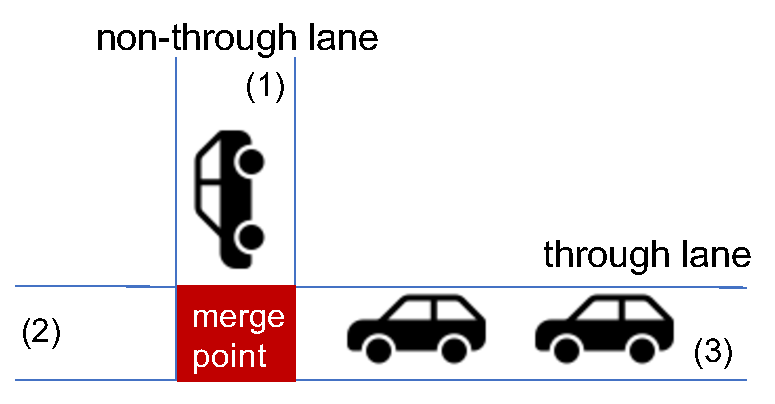
\includegraphics{Pictures/merge_point.pdf}}
\end{center}
\caption{Merge point}
\label{mergePoint_fig}
\end{figure}

S. Aoki and R. Rajkumar~\cite{10.1145/3055004.3055028} have proposed a
merging protocol for autonomous vehicles. The protocol has two
versions that correspond to two traffic environments: (1) only
autonomous vehicles on the traffic (homogeneous traffic) and (2)
autonomous vehicles and human-driven vehicles on the traffic
(heterogeneous traffic).  In the present paper, we only concentrate on
the first version (1) which is called the Aoki-Rajkumar merging
protocol or simply the AR merging protocol.  The protocol requires
each vehicle to be equipped with software systems, such as a
navigation system with hardware devices, such as sensors.  Furthermore,
the authors also assume that each vehicle is able to use some
technologies, such as WAVE \cite{4346439,5888501}, and GPS, to
communicate with other vehicles.

All vehicles participating in the protocol are controlled based on two
system modes: prioritized mode and fair mode.  When the system is in
one mode, it can change to the other mode depending on the traffic of
the through lane. Each mode is explained in the upcoming sub-sections.

\subsection{Prioritized mode}

When the system is in prioritized mode, non-through lane vehicles
basically cannot intervene through lane vehicles that are approaching
the merge point.  It means that non-through lane vehicles are allowed
to enter the merge point only if there is no through lane vehicle that
is approaching the merge point.  There are basically two cases:

\begin{itemize}
\item if there are some through lane vehicles that are approaching the
  merge point and there is not enough space between any of two adjacent
  such vehicles, non-through lane vehicles must stop before the merge
  point until all such through lane vehicles have passed through the
  merge point;

\item if there is no through-lane vehicle that is approaching the
  merge point, non-through lane vehicles are allowed to pass through
  the merge point.
\end{itemize}

\noindent
There is actually one more case:

\begin{itemize}
\item if there are some through lane vehicles that are approaching the
  merge point and there is enough space between some of two adjacent
  such vehicles, non-through lane vehicles can use the space to enter
  the merge point.
\end{itemize}

\noindent
In the AR merging protocol~\cite{10.1145/3055004.3055028}, prioritized
mode is classified into fully prioritized mode and half prioritized
mode that correspond to the first two cases and the third case,
respectively. 

% \begin{figure}[h]
% \begin{center}
% \scalebox{0.33}{\includegraphics{Pictures/fullyPrioritized.pdf}}
% \end{center}
% \caption{Fully-prioritized state}
% \label{fullyPri_fig}
% \end{figure}


%\subsection{Semi-prioritized mode}
%\label{semi-case}
%
%When the system is in semi-prioritized mode, non-through lane vehicles
%have a chance to enter the merge point even though there are some
%through lane vehicles that are approaching the merge point.  If there
%is enough space between two through lane vehicles that are approaching
%the merge point, a non-through lane vehicle that is approaching the
%merge point can use that space to enter the merge point.
%
% \begin{figure}[h]
% \begin{center}
% \scalebox{0.33}{\includegraphics{Pictures/semiPrioritizedNonthrough.pdf}}
% \end{center}
% \caption{Fully-prioritized state}
% \label{semiPriNT}
% \end{figure}

\subsection{Fair mode}

Prioritized mode can change to fair mode when the traffic of the
through lane becomes congested. In fair mode, through lane vehicles
and non-though lane vehicles are allowed to enter the merge point
alternately. Fair mode can change back to prioritized mode when the
traffic of the through lane becomes less congested.

\subsection{Part of the pseudo-code}

Due to the space limitation, we cannot describe the AR merging
protocol in pseudo-code in detail. Let us show part of the pseudo-code:

\begin{small}
\begin{tabbing}
\=\ \ \ \ \=\ \ \=\kill
\>\>\textbf{else if} $\textrm{RM}(\omega_{l1}) = \textrm{APPROVE}$ \textbf{then} \\
\>\>\>Start the maneuver; \\
\>\>\textbf{else if} $\textrm{Average}\{\upsilon_{\omega_{h1}},\ldots,\upsilon_{\omega_{hn}}\}  < \psi$ \textbf{then} \\
\>\>\>$\textrm{SM}(\omega_{h1}) = \textrm{ENTER}$; \\
\>\>\>\ldots
\end{tabbing}
\end{small}

\noindent
This says the following: if the top non-thourgh lane vehicle
$\omega_{l1}$ receives the message $\textrm{APPROVE}$ from a through
lane vehicle, then $\omega_{l1}$ enters the merge point; if the
average speed of the multiple thorugh lane vehicles
$\upsilon_{\omega_{h1}},\ldots,\upsilon_{\omega_{hn}}$ is less than
$\psi$, $\omega_{l1}$ sends the message $\textrm{Average}$ to the top
through lane vehicle $\omega_{h1}$.

% \begin{figure}[t]
% \begin{center}
% \scalebox{0.33}{\includegraphics{Pictures/fairState.pdf}}
% \end{center}
% \caption{Fair state}
% \label{semiPriNT}
% \end{figure}




% Algorithm 1, Algorithm 2 and Algorithm 3 present the algorithm of \textit{Autonomous Vehicle Protocol for Merge Points}. Algorithm 1 presents the protocol for the vehicle on the non-through lane, and Algorithm 2 presents the protocol for the vehicle on the through lane. In addition, Algorithm 3 presents the protocol for the vehicle on the non-through lane when the vehicle is in Fair state. The vehicles on the non-through lane, originally having the lower priority which are represented by $\omega_{l1}$, .. $\omega_{ln}$. The vehicles on the through lane originally having higher priority are denoted as $\omega_{h1}$, ... $\omega_{hn}$. The sequential subscript numbers indicate the vehicle order, meaning $\omega_{l1}$ is the leader vehicle on the non-through lane before the merge intersection.



% The CROSS message is not used in any algorithms because this perception is sufficiently safe for the intersection. However, it is used in order to enhance the reliability and safety of the protocol.


% \begin{algorithm}[t]
% \caption{Protocol for Vehicle $\omega_{l1}$ on non-through lane} 
% \label{alg:nlane}
% \While{\textit{not started the maneuver}}
% {
% SM( $\omega_{l1}$) = \textbf{REQUEST};\newline
% \uIf{\textit{not halting before the merge point}}
% {
% \uIf{\textit{No vehicle before the merge point}}{Start the maneuver;}
% \uElseIf{\textup{RM($\omega_{l1}$) = \textbf{APPROVE}}}{Start the maneuver;}
% \Else{Slow down (for halting right before the merge point);}
% }
% \Else{
% Halting before the merge point($\upsilon_{\omega_{h1}}$ = 0);\newline
% \uIf{\textit{not halting before the merge point}}{Start the maneuver;}
% \uElseIf{\textup{RM($\omega_{l1}$) = \textbf{APPROVE}}}{Start the maneuver;}
% \uElseIf{Average\{$\upsilon_{\omega_{h1}}$,..$\upsilon_{\omega_{hn}}$\}  $<$ $\psi$}
% {SM($\omega_{h1}$) = \textbf{ENTER};\newline
% SM($\omega_{l2}$, ..$\omega_{ln}$) = \textbf{STATE TRANSITION};\newline
% $\omega_{h1}$  transits to \textit{Fair state};\newline
% Start the maneuver;
% }
% \Else{
% \textit{k} = arg max \textit{D\{$\omega_{hi}$\}};\newline
% SM($\omega_{hk}$) = \textbf{INTERRUPT};\newline
% \If{\textup{RM($\omega_{hk}$) = \textbf{YIELD}}}
% {
% \While{$s_{1}$ sec}
% {
% \If{\textup{RM($\omega_{h(k-1)}$ = \textbf{EXIT}}}{Start the maneuver;}
% }
% }
% }
% }
% }
% \end{algorithm}


% Some other notations used in these algorithms.
% \begin{itemize}
%     \item $\upsilon_{\omega_{hk}}$: Current speed of the vehicle $\omega_{hk}$
%     \item $\psi$: Speed threshold
%     \item $s_{1}$: Time threshold for packet loss (for \textbf{INTERRUPT} or \textbf{YIELD})
%     \item $s_{2}$: Time threshold for packet loss (for \textbf{EXIT)}
%     \item $\Delta$: Time threshold for \textbf{ABOUT TO EXIT}
% \end{itemize}


% \begin{algorithm}[t]
% \caption{Protocol for Vehicle $\omega_{h1}$ on through lane}
% \label{alg:tlane}
% \uIf{RM($\omega_{h1}$) = \textbf{\textup{REQUEST}}}
% {
% \uIf{CollisionDetect($\omega_{h1}$, $\omega_{l1}$) = true}
% {SM($\omega_{l1}$) = \textbf{DECLINE};\newline Start the maneuver;}
% \Else{SM($\omega_{l1}$) = \textbf{APPROVE};\newline Start the maneuver;}
% }
% \uElseIf{RM($\omega_{h1}$) = \textbf{\textup{ENTER}}}
% {
% \While{$s_2$sec}
% {
% \uIf{RM($\omega_{l1}$) = \textbf{\textup{ABOUT TO EXIT}}}{
% SM($\omega_{l1}$) = \textbf{ENTER};\newline
% Going to start the maneuver;\newline
% \uIf{RM($\omega_{l1}$) $\neq$ \textbf{\textup{EXIT}} in $\Delta$sec later after \textbf{\textup{ABOUT TO EXIT}}}{Slow down and Halting;}
% \Else{Start the maneuver;}
% }
% \uElseIf{RM($\omega_{l1}$) = \textbf{\textup{EXIT}}}{Start the maneuver;}
% \Else{Halting;}
% }
% \uIf{No vehicle before the merge point}{Start the maneuver;}
% \Else{Halting;}
% }
% \uElseIf{RM($\omega_{l1}$) = \textbf{\textup{INTERRUPT}}}{\uIf{CollisionDetect($\omega_{h1}$, $\omega_{l1}$) = true}{Slow down(to make space for $\omega_{l1}$);\newline
% SM($\omega_{l1}$) = \textbf{YIELD};}
% \Else{SM($\omega_{l1}$) = \textbf{YIELD};}}
% \Else{Start the maneuver;}
% \end{algorithm}

% \begin{algorithm}[t]
% \caption{Protocol for Vehicle $\omega_{l1}$ in Fair state}
% \label{alg:fair}
% \uIf{right before the merge point}{
% \uIf{RM($\omega_{h1}$) = \textbf{\textup{ABOUT TO EXIT}}}{
% SM($\omega_{h2}$) = \textbf{ENTER};\newline
% SM($\omega_{l2}$, ..$\omega_{ln}$) = \textbf{STATE TRANSITION};\newline
% Going to start the maneuver;\newline
% \uIf{RM($\omega_{h1}$) $\neq$ \textbf{\textup{EXIT}} in $\Delta$sec later after \textbf{\textup{ABOUT TO EXIT}}}{Halting;}
% \Else{Start the maneuver;}
% }
% \uElseIf{RM($\omega_{h1}$) = \textbf{\textup{EXIT}}}{
% SM($\omega_{h2}$) = \textbf{ENTER};\newline
% SM($\omega_{l2}$, ..$\omega_{ln}$) = \textbf{STATE TRANSITION};\newline
% Start the maneuver;
% }
% \Else{Halting;}
% }
% \Else{Follow the vehicle in front;}
% \end{algorithm}

% In the \textit{Autonomous Vehicle Protocol for Merge Points}, three functions implies three priority state of non-through lane vehicles. (i)High throughput function; (ii) Intervention function; (iii) Zipper merge function. 


\section{A Revised Version of the Protocol}
 \label{sect_reviproto}

We revise the AR merging protocol such that it does not rely on any
real-time information, such as the average speed of multiple vehicles
running on a lane. Or we can say that we design a new merging protocol
that does not rely on such information based on the AR merging
protocol. Because the speed of a vehicle may drastically change in a
short moment, say by sudden breaking, we do not think that the average
speed of multiple vehicles is reliable enough to safely control
autonomous vehicles. The revised version of the AR merging protocol is
called our merging protocol (or our protocol) in the present paper.
Each vehicle in our protocol is attached to one of five statuses:
\textit{running}, \textit{approaching}, \textit{stopped},
\textit{crossing}, or \textit{crossed}.  When a vehicle
is far away from the merge point, its status is running. When a
vehicle gets close to the merge point, its status changes to
approaching from running. When a vehicle stops before the merge point,
its status is stopped. When a vehicle enters the
merge point, its status changes to crossing from approaching or stopped. 
When a vehicle has passed through the merge point, its
status changes to crossed from crossing. We suppose that vehicles
whose statuses are approaching, or stopped on one lane never
pass over any other vehicles. We use a boolean variable to check whether
the vehicle is in the merge point or not. To this end, we need to use V2V
communications. Such vehicles can be regarded as making a virtual
queue of vehicles. As the AR merging protocol, there are two modes
(prioritized mode and fair mode) in our protocol. Initially,
we suppose that the system is in prioritized mode, the boolean variable is false
and each vehicle is in running.

In our protocol, there are three cases in which a non-through lane
vehicle is allowed to enter the merge point: (i) no through lane
vehicle is approaching the merge point (prioritized mode); (ii) some through lane
vehicles are approaching the merge point such that there is enough
space between some two adjacent vehicles (prioritized or fair mode); (iii) through lane and
non-through lane vehicles enter the merge point alternately when the
traffic of the through lane is congested (fair mode).

\begin{figure}[h]
\begin{center}
\scalebox{0.36}{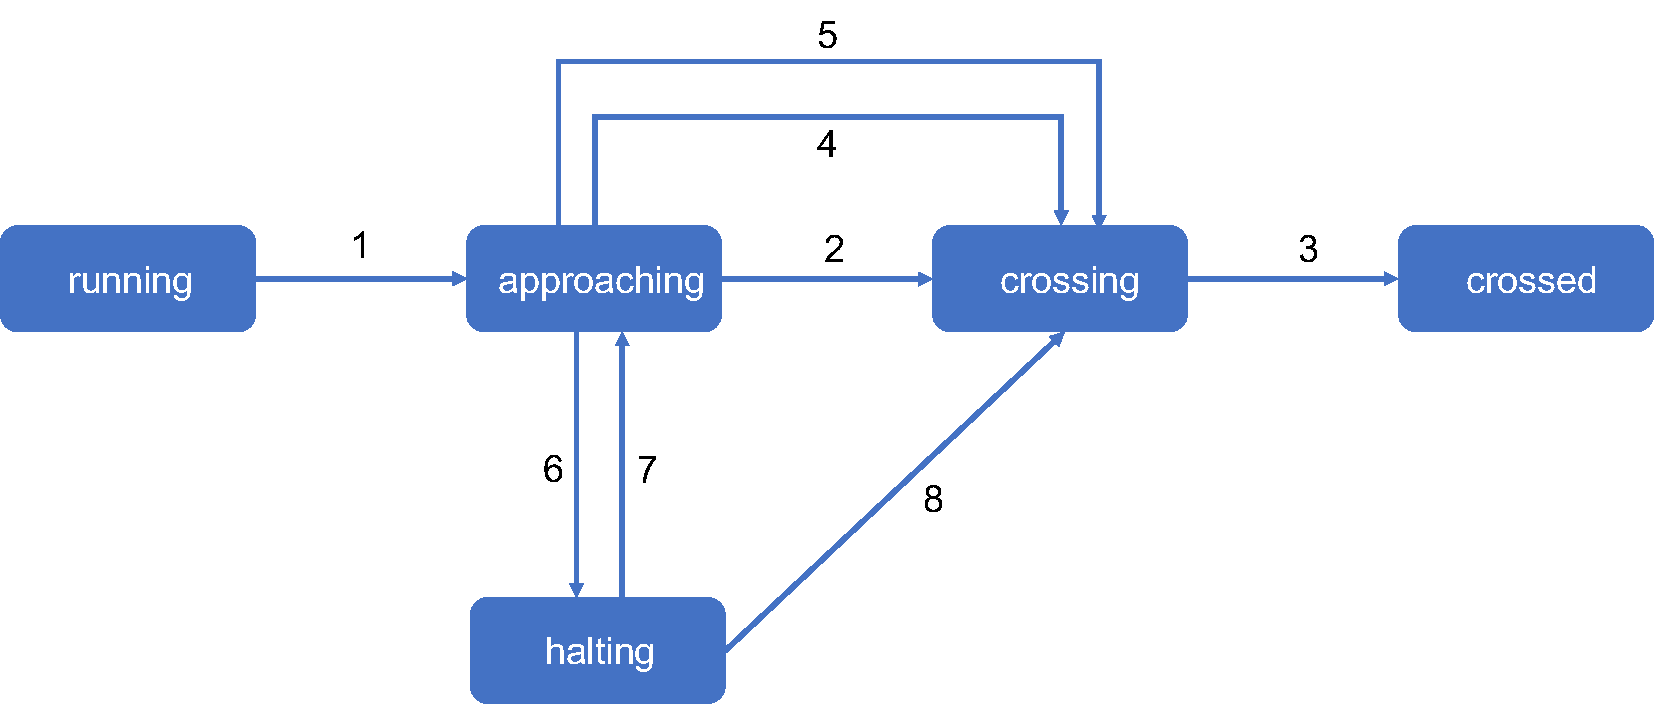
\includegraphics{Pictures/throughLane.pdf}}
\end{center}
\caption{Transition of a through lane vehicle's status}
\label{throughLaneStatus}
\end{figure}

Fig.~\ref{throughLaneStatus} visualizes the change of the status
of a through lane vehicle.  Each arrow represents the change of the
vehicle status from one value to another if the condition (or the
trigger event) denoted by the number attached to the arrow is
satisfied.  Each condition (or trigger event) is:
\begin{itemize}[]
    \item[1)] The vehicle gets close to the merge point. %1
    \item[2)] Some vehicle is in the merge point. %2
    \item[3)] The system is in fair mode and there is non-through lane vehicle's turn. %3
    \item[4)] The system is in prioritized mode. The vehicle either approaching or stopped 
    can enter the merge point. %4
    \item[5)] The system is in fair mode and through lane vehicle's turn. The vehicle either 
    approaching or stopped can enter the merge point. %5
    \item[6)] The system is in prioritized mode. %6
    \item[7)] The system is in fair mode and there exists a non-through lane vehicle approaching the 
    merge point. %7
    \item[8)] No vehicle on non-through lane.
    \item[1')] A space appears in through lane. %1' 
    \item[2')] A space is a top element of through lane, and there exists some vehicle 
    is in non-through lane. %2' 
    \item[3')] Some space is top element of through lane. %3'
\end{itemize}

When a system is in fair mode (or the traffic is congested), the number of the through lane
vehicles that constitute the virtual queue on the through lane is
greater then a specific number. Otherwise, the system is in prioritized mode.
Note that the through lane vehicles that constitute the virtual queue on the
through lane are in approaching or stopped or crossing.
It refers that only the through lane vehicles that constitute the virtual queue
on the through lane can affect the system. Furhtermore, we also define two turns 
for through and non-through lane vehicle in the fair mode.

Fig.~\ref{space} visualizes two cases that a non-through lane vehicle can enter
the merge point when the top of the through lane is a space.
The blue circle
represents the non-through lane vehicle, the red circle represents the
through lane vehicles, and the white circle represents a space. The green
area denotes the merge point. Each vehicle or space is attached to a
different number.
A non-through lane vehicle whose status is approaching or stopped on the top through lane
can enter the merge point even the system is in prioritized or fair mode.
Let us note that space is only used in through lane.

\begin{figure}[h]
	\begin{center}
		\scalebox{0.28}{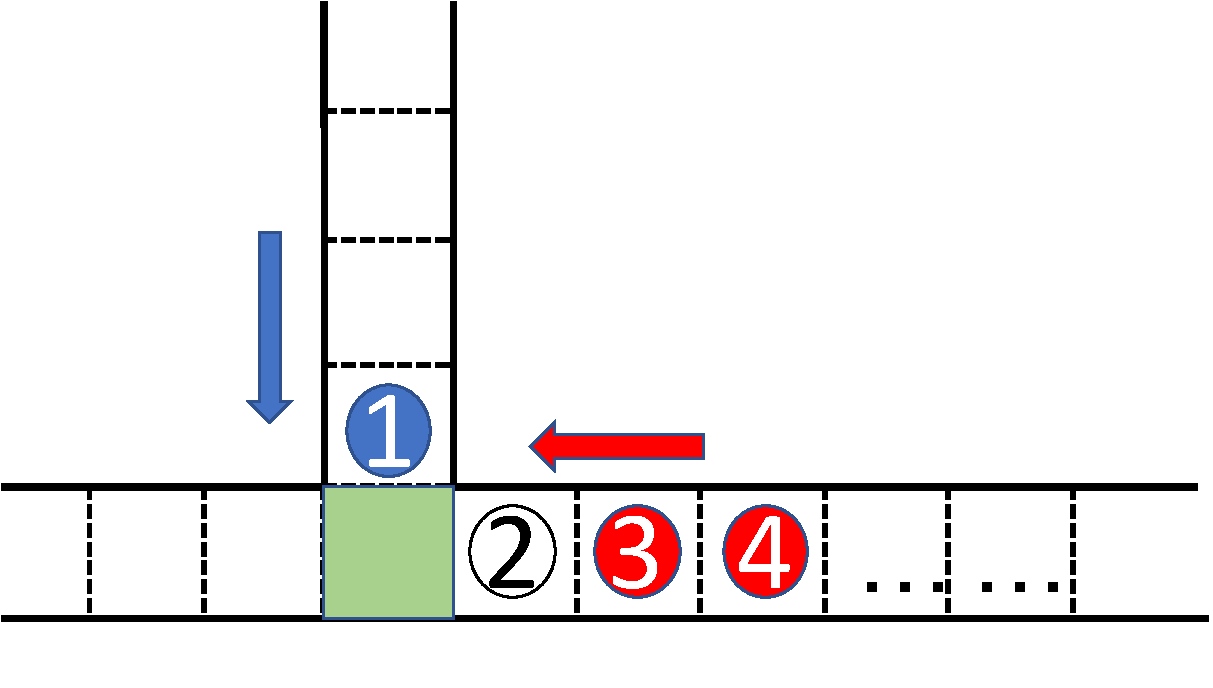
\includegraphics{Pictures/space.pdf}}
	\end{center}
	\caption{Two cases for the non-through lane vehicle entering the merge point}
	\label{space}
\end{figure}

\begin{figure}[h]
\begin{center}
\scalebox{0.36}{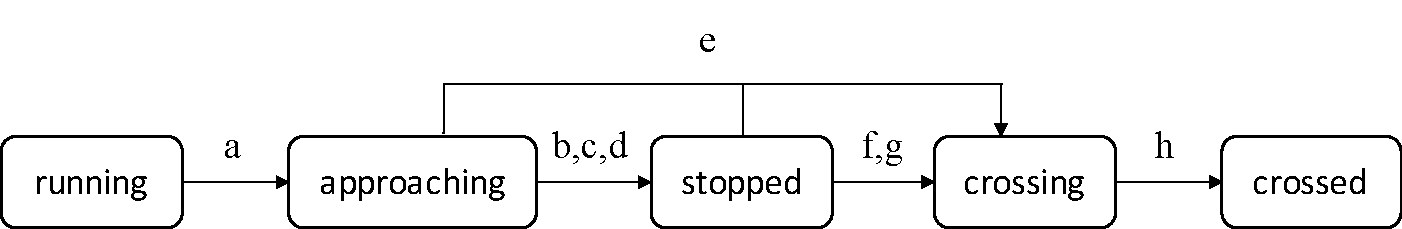
\includegraphics{Pictures/nonThroughLane.pdf}}
\end{center}
\caption{Transition of a non-through lane vehicle's status}
\label{nonThroughLaneStatus}
\end{figure}

Fig.~\ref{nonThroughLaneStatus} visualizes the change of the status
of a non-through lane vehicle.  Each arrow represents the change of the
vehicle status from one value to another if the condition (or the
trigger event) denoted by the character attached to the arrow is
satisfied.  Each condition (or trigger event) is:

\begin{itemize}
  \item[a)] The vehicle gets close to the merge point. 
  \item[b)] Some vehicle is in the merge point. 
  \item[c)] The system is in fair mode and there is through lane vehicle's turn. 
  \item[d)] The system is in prioritized mode and no vehicle on through lane. The vehicle either 
  approaching or stopped can enter the merge point.
  \item[e)] The system is in fair mode and non-through lane vehicle's turn. The vehicle either 
  approaching or stopped can enter the merge point. 
  \item[f)] The top of through lane is space (refer to condition 2'). 
  \item[g)] The system is in prioritized mode.
  \item[h)] The system is in fair mode. 
\end{itemize}

Note that the non-through lane vehicles do not affect the mode of the system even
some vehicle is in the merge point.
The details of all conditions will be mentioned in the following section.

 
\section{Formal Specification}
 \label{sect_formal}
We use two queues to maintain the vehicles running on the through lane and non-through lane, respectively.
In the through lane, each element in the queue can be either a vehicle or a space.
In this paper, a state is expressed as a soup of observable components.
To formalize the protocol, we use four observable components as follows:
\begin{itemize}
  \item (\verb!v[!$id$\verb!]:!$position$\verb!,!$vstat$) - $id$ is an ID (a nature number) of 
  a vehicle or a space (we assume that if the ID is less than 100, it represents a vehicle, otherwise it 
  represents a space), 
  $position$ is the lane that the vehicle, or the space (only on through lane) $id$ is located, 
  $vstate$ is the status of the vehicle if it is a 
  vehicle. Initially, $vstate$ is \verb!unspace! if it is a space, or \verb!running! if it is a vehicle.
  \item (\verb!lane[!$position$\verb!]:!$q$) - $position$ is the through lane or 
  non-through lane, and $q$ is a queue of vehicles and spaces (only on through lane). 
  Initially, $q$ is \verb!empq!, which denotes an empty queue.
    
  \item (\verb!vehicleCrossing:!$b$) - $b$ is either true or false, indicating that there 
  exists a vehicle crossing the merge point or there does not, respectively. Initially, $b$ is false.
  
  \item (\verb!mode:!$smode$) - $smode$ receives one of the following three values: 
  \verb!prioritized! indicating that the system is in prioritized mode, 
  \verb!fairT! indicating that the system is in fair mode and it is the through lane vehicle's turn,
  \verb!fairN! indicating that the system is in fair mode and it is the non-through lane vehicle's turn.
  
  Initially, $smode$ is \verb!prioritized!.
  
  \item (\verb!gstat! : $gstat$) -  $gstat$ is either \verb!fin! or \verb!nFin!.
  When it is \verb!fin!, all vehicles concerned have crossed the intersection.
\end{itemize}

We define a function that counts the number of the through lane
vehicles that constitute the virtual queue to check whether the 
traffic is congested as follows:
\begin{small}
\begin{verbatim}
op #(_,_,_) : Queue Nat Nat -> Nat .
eq #(empq, X, Y) = X .
eq #(Q, X, 0) = X .
ceq #((Z ; Q), X, Y) = #(Q, X, sd(Y,1)) 
                if Z >= 100 .
ceq #((Z ; Q), X, Y) = #(Q, s(X), sd(Y,1)) 
                if Z < 100 .
\end{verbatim}
\end{small}
\noindent where \verb!Q!, \verb!X!, \verb!Y!, \verb!Z! are Maude variables 
for queue and three natural numbers, respectively. \verb!sd()!, \verb!s()! are 
Maude operations for decrementing and incrementing, respectively.
This function returns the number of vehicles of top \verb!Y! elements of the queue
in which \verb!Y! is set to five in our specificaiton. 
 
We use 15 rewrite rules to define the transitions of the protocol mentioned in \ref{sect_reviproto}.
Those rewrite rules are divided into four groups: vehicles get close to the merge point,
the vehicle stops before the merge point, the vehicle is in the merge point and 
the vehicle crossed the merge point.

\subsection{Vehicles approach the merge point}
The following rules refers to conditions 1), a), and 1'), respectively:
\begin{small}
  \begin{verbatim}
crl [approach_T] : 
{(mode: M) (lane[L]: VS) 
 (v[VI]: L,running) OCs} 
  => {(mode: (if (#(VS,0,5) >= 3 
            and M == prioritized) 
            then fairT else M fi))
  (lane[L]: (VS ; VI)) 
  (v[VI]: L,approaching) OCs} 
if L == through .

crl [approach_N] : 
  {(lane[L]: VS) (v[VI]: L,running) OCs} 
  => {(lane[L]: (VS ; VI)) 
    (v[VI]: L,approaching) OCs} 
if L == noThrough .

crl [approach_space] : 
  {(lane[L]: VS) (v[VI]: L,unspace) OCs} 
=> {(lane[L]: (VS ; VI)) 
    (v[VI]: L,space) OCs} 
if L == through .
  \end{verbatim}
\end{small}

\noindent where \verb!M!, \verb!L!, \verb!VS!, and \verb!VI! 
are Maude variables for mode, lane information (through or non-through), queue, and vehicle ID, respectively.
\verb!OCs! is a Maude variable for observer components.
\verb!#(VS,0,5) >= 3! checks the traffic when there are at least three
vehicles of top five elements in the queue, it is congested, otherwise 
it is prioritized. Let us repeat that only through lane vehicles affect
to the mode so when space is put into queue, it does not change the mode.
Those rewrite rules change the status of the vehicle or space when they are put into queue.

\subsection{Vehicles stop before the merge point}
The following rewrite rules refer to conditions 2), 3), b), and c) in which 
rewrite rule \verb!stopped! corresponds to 2), and b), rewrite rule 
\verb!fair_T_stopped! corresponds to 3), and \verb!fair_N_stopped! corresponds
to c).
\begin{small}
  \begin{verbatim}
rl [stopped] : 
 {(vehicleCrossing: true) (lane[L]: (VI;VS)) 
  (v[VI]: L,approaching) OCs} 
=> {(vehicleCrossing: true) 
    (lane[L]: (VI;VS)) 
    (v[VI]: L,stopped) OCs} .

crl [fair_T_stopped] : 
 {(mode: fairN) (lane[through]: (VI;VS)) 
  (v[VI]: through,approaching) 
  (lane[noThrough]: (VI' ; VS')) 
  (v[VI']: noThrough,VeSt) OCs} 
=> {(mode: fairN) (lane[through]: (VI;VS)) 
    (v[VI]: through,stopped)
    (lane[noThrough]: (VI';VS')) 
    (v[VI']: noThrough,VeSt) OCs} 
if (VeSt == approaching or VeSt == stopped) .

crl [fair_N_stopped] : 
 {(mode: M) (lane[through]: (VI;VS)) 
  (v[VI]: through,VeSt) 
  (lane[noThrough]: (VI';VS')) 
  (v[VI']: noThrough, approaching) OCs} 
=> {(mode: M) (lane[through]: (VI;VS)) 
    (v[VI]: through,VeSt)
    (lane[noThrough]: (VI';VS')) 
    (v[VI']: noThrough,stopped) OCs} 
if (M =/= fairN) /\ (VeSt == approaching 
                    or VeSt == stopped) .    
  \end{verbatim}
\end{small}

\noindent where \verb!VeSt! is a Maude variable for vehicle status.
The rewrite rules say that if some vehicle is in the merge point,
the status of top vehicle on both lane changes to \textit{stopped}.
If the system is in fair mode and it is through lane vehicle's turn,
the top of non-through lane changes to \textit{stopped}. For the case 
non-through lane vehicle's turn, it works similarlly.
For non-through lane vehicles, there has one more case such that the system
is in prioritized mode, if there exists one vehicle on through lane, 
the non-through lane vehicle must stop.

\subsection{Vehicle enters the merge point}
The following rewrite rules refer to conditions 2', 3', 4), 5), d), e), and f)
in which \verb!prioritized_T_crossing! corresponds to 4) and 5), \verb!prioritized_N_crossing!
corresponds to d), \verb!fair_N_crossing! corresponds to e), \verb!N_space! 
corresponds to f) and 2'), and \verb!del_space! refers to 3'.

\begin{small}
  \begin{verbatim}
crl [prioritized_T_crossing] : 
 {(vehicleCrossing: false) (mode: M) 
  (lane[through]: (VI ; VS)) 
  (v[VI]: through,VeSt) OCs} 
=> {(vehicleCrossing: true) (mode: M) 
  (lane[through]: (VI ; VS)) 
  (v[VI]: through,crossing) OCs} 
if (M =/= fairN) /\ (VeSt == approaching 
                  or VeSt == stopped) .

crl [prioritized_N_crossing] : 
 {(vehicleCrossing: false) 
  (mode: prioritized) 
  (lane[through]: empq) (lane[L]: (VI ; VS)) 
  (v[VI]: L,VeSt) OCs} 
=> {(vehicleCrossing: true) 
  (mode: prioritized) 
  (lane[through]: empq) (lane[L]: (VI ; VS)) 
  (v[VI]: L,crossing) OCs}
if L == noThrough /\ (VeSt == approaching 
                   or VeSt == stopped) .

crl [fair_N_crossing] : 
 {(vehicleCrossing: false) (mode: fairN) 
  (lane[L]: (VI ; VS)) (v[VI]: L,VeSt) OCs} 
=> {(vehicleCrossing: true) (mode: fairN) 
  (lane[L]: (VI ; VS)) (v[VI]: L,crossing) 
  OCs} 
if L == noThrough /\ (VeSt == approaching 
                   or VeSt == stopped) .

crl [N_space] : 
 {(vehicleCrossing: false) (mode: M)
  (lane[through]: (VI ; VS)) 
  (v[VI]: through,space) 
  (lane[noThrough]: (VI' ; VS')) 
  (v[VI']: noThrough,VeSt) OCs} 
=> {(vehicleCrossing: true) 
 (mode: (if (#(VS,0,5) >= 3 and 
 M == prioritized) then fairT else M fi))
  (lane[through]: VS) 
  (v[VI]: through,yield)
  (lane[noThrough]: (VI' ; VS')) 
  (v[VI']: noThrough,crossing) OCs}
if (VeSt == approaching or VeSt == stopped) .

rl [del_space] : 
 {(mode: M) (lane[through]: (VI ; VS)) 
  (v[VI]: through,space) OCs} 
=> {(mode: (if (#(VS,0,5) >= 3 and 
 M == prioritized) then fairT else M fi))
  (lane[through]: VS) 
  (v[VI]: through,yield) OCs} .
  \end{verbatim}
\end{small}

Let us consider the rewrite rule \verb!N_space!, it is a case such that
the top element of the through lane is space, then if there exists a 
non-through lane vehicle, it can enter the merge point. After that, 
the space is removed. Note that, we update the mode because the queue
on through lane has been modified. The rewrite rule \verb!del_space! deletes 
the top element of through lane and update the mode.
The other rewrite rules work similarly.

\subsection{Vehicle crossed the merge point}
The following rewrite rules refers to remaining transitions 6),7),8), g), and h) in which
\verb!prioritized_crossed! corresponds to 6) and g), \verb!N_crossed! corresponds to h),
\verb!fair_T_crossed1! corresponds to 7), and \verb!fair_T_crossed2! corresponds to 8).

\begin{small}
  \begin{verbatim}
rl [prioritized_crossed] : 
 {(vehicleCrossing: true) 
  (mode: prioritized) 
  (lane[L]: (VI ; VS)) 
  (v[VI]: L,crossing) OCs} 
=> {(vehicleCrossing: false) 
  (mode: prioritized) 
  (lane[L]: VS) 
  (v[VI]: L,crossed) OCs} .

crl [N_crossed] : 
 {(vehicleCrossing: true) (mode: M) 
  (lane[L]: (VI ; VS)) 
  (v[VI]: L,crossing) OCs} 
=> {(vehicleCrossing: false) (mode: fairT) 
  (lane[L]: VS) (v[VI]: L,crossed) OCs} 
if (L == noThrough) /\ (M =/= prioritized) .

crl [fair_T_crossed1] : 
  {(vehicleCrossing: true) (mode: fairT) 
  (lane[through]: (VI ; VS)) 
  (v[VI]: through,crossing) 
  (lane[noThrough]: (VI' ; VS')) 
  (v[VI']: noThrough,VeSt) OCs} 
=> {(vehicleCrossing: false) 
  (mode: (if (#(VS,0,5) >= 3) 
   then fairN else prioritized fi))
  (lane[through]: VS) 
  (v[VI]: through,crossed)
  (lane[noThrough]: (VI' ; VS')) 
  (v[VI']: noThrough,VeSt) OCs} 
if (VeSt == approaching or VeSt == stopped) .

rl [fair_T_crossed2] : 
  {(vehicleCrossing: true) (mode: M)
  (lane[through]: (VI ; VS)) 
  (v[VI]: through,crossing) 
  (lane[noThrough]: empq) OCs} 
=> {(vehicleCrossing: false) 
  (mode: (if (#(VS,0,5) >= 3) 
   then fairT else prioritized fi))
  (lane[through]: VS) (v[VI]: through,crossed) 
  (lane[noThrough]: empq) OCs} .    
  \end{verbatim}
\end{small}
 
In prioritized mode (\verb!prioritized_crossed!), both lane do not affect the mode so we only
update the vehicle's status.
In fair mode (\verb!N_crossed!), \verb!FairT! is set for non-through lane vehicle even 
it is through lane vehicle's turn or non-through lane vehicle's turn.
Note that the non-through lane vehicle can enter the merge point in 
through lane vehicle's turn when condition f) or 2') is satisfied.

Let us consider the rewrite rule \verb!fair_T_crossed1! (in case the condition
7) is satisfied), we check the traffic except for the vehicle in the merge point.
If it is still congested, the mode is updated to non-through lane vehicle's turn,
otherwise, the system returns to prioritized mode. In the rewrite rule 
\verb!fair_T_crossed2! based on condition 8), we update the \verb!mode! by checking the 
traffic except for the vehicle in the merge point.
The update of the system is same as the rewrite rule \verb!fair_T_crossed1!.
Please go to the webpage shown in the Sect.~\ref{sect_intro} to read fully our specification.
 


 
\section{Model Checking}
\label{sect_model}
There are three desired properties the \textit{a-merging} protocol should enjoy:
\begin{itemize}
    \item \textit{Mutual exclusion} - There is at most one vehicle crossing the merge point at any given time.
    \item \textit{Deadlock freedom} - There is no deadlock state.
    \item \textit{Starvation freedom} - If a vehicle is trying to cross the merge point, then the vehicle must eventually pass the merge point.
\end{itemize}

%We need an initial state that can cover all three states in our \textit{Revised Autonomous Vehicle Protocol for Merge Points}.
%Therefore, we put two spaces and three vehicles on the through lane, one space and three vehicles on the non-through lane.
%To cover all situations (three states) in the \textit{a-merging} protocol, we assume that two spaces and three vehicles on the through lane, one space and three vehicles on the non-through lane.
%The \verb!init! is shown as follows:

We experiment that there are three vehicles on the non-through lane,
four vehicles and two spaces on the through lane.
The initial state namely \verb!init! is defined as follows:
\begin{small}
\begin{verbatim}
{(gstat: nFin) (vehicleCrossing: false) 
(mode: prioritized) (lane[through]: empq) 
(lane[noThrough]: empq) 
(v[101]: through,unspace) 
(v[102]: through,unspace)
(v[1]: noThrough,running) 
(v[2]: noThrough,running) 
(v[3]: noThrough,running)
(v[4]: through,running) 
(v[5]: through,running) 
(v[6]: through,running) 
(v[7]: through,running) } .
\end{verbatim}
\end{small}

\subsection{Mutual exclusion}

The \textit{mutual exclusion} property can be checked by the following search commmand:

\begin{small}
\begin{verbatim}
search [1] in MERGING : 
init =>* {(v[VI]: LN, crossing) 
(v[VI']: LT, crossing) OCs} 
            such that VI =/= VI' .
\end{verbatim}
\end{small}

\noindent
where \verb!MERGING! is the specification of our protocol, \verb!LN! and \verb!LT!
are Maude variables for lane information.
The search commands tries to find a state from the initial state \verb!init! 
such that two different vehicles are crossing the merge point simultaneously.
Maude finished without finding any such a state.
It confirms that when there are seven vehicles and two spaces participating, the protocol 
enjoys the \textit{mutual exclusion} property with the case \verb!init!.

\subsection{Deadlock freedom}
To check that there is no deadlock state, we use the following command:

\begin{small}
\begin{verbatim}
search [1] in MERGING : init =>! {OCs} .
\end{verbatim}
\end{small}

\noindent
No state was found. It confirms that the initial state has no deadlock.


\subsection{Starvation freedom}
To model check that the protocol enjoys the \textit{starvation freedom} property, 
we need to employ Maude LTL model checking facilities.

We first define two atomic propositions namely \verb!want! and \verb!passed! 
which takes a vehicle IDs as their argument. 
They are defined via the following equations:

\begin{small}
\begin{verbatim}
eq {(v[VI]: L,approaching) OCs} |= 
  want(VI) = true .
eq {(v[VI]: L,crossed) OCs} |= 
  passed(VI) = true .
eq {OCs} |= PROP = false [owise] .
\end{verbatim}
\end{small}

\noindent
where \verb!PROP! is a Maude variable of atomic propositions, 
\verb!|=! is a Maude symbol for satisfaction relation in LTL,
\verb!owise! is the abbreviation of otherwise, indicating that 
this equation will only be applied if all of the previous 
equations above it cannot be applied. 
The equations say that \verb!want(VI)! holds in a state $s$ iff $s$ 
contains \verb!(v[VI]: L,approaching)!, which means that the vehicle 
\verb!VI! is trying to enter the merge point. 
Likewise, \verb!passed(VI)! holds in a state $s$ iff $s$ contains 
\verb!(v[VI]: L,crossed)!, which means that the vehicle \verb!VI! 
already passed the merge point. 

The \textit{starvation freedom} property for each vehicle is then 
defined by the LTL formula \verb!lofree0! as follows:

\begin{small}
\begin{verbatim}
eq lofree0(VI) = (want(VI) |-> passed(VI)) .
\end{verbatim}
\end{small}

\noindent
The formula says that if a vehicle \verb!VI! trying to cross the merge point, 
it eventually will pass through the merge point.
After that, the complete \textit{starvation freedom} property is specified 
by the LTL formula \verb!lofree! as follows:

\begin{small}
\begin{verbatim}
eq lofree = lofree0(1) /\ lofree0(2) /\ 
				lofree0(3) /\ lofree0(4) /\ 
				lofree0(5) /\ lofree0(6) /\ lofree0(7) .
\end{verbatim}
\end{small}

The following command is used to model check the property:
\begin{small}
\begin{verbatim}
red in MERGING-CHECK : 
        modelCheck(init,lofree) .
\end{verbatim}
\end{small}

\noindent
No counterexamples were found. 
Consequently, we can conclude that the protocol enjoys the \textit{starvation freedom} 
property with seven vehicles and two spaces participating in the protocol.
 
\section{Related Work}
 \label{sect_Relate}
 
An autonomous vehicle intersection control protocol called LJPL protocol has 
been proposed to handle the mutual exclusion property in the intersection~\cite{LimJongBeom2018Aedm}.
The authors design two type of lanes: concurrent and conflict lanes. 
The protocol allows that the vehicles on concurrent lanes can enter the 
intersection simultaneously while the vehicles on conflict lanes cannot 
enter the intersection simultaneously.
The intersection in the LJPL protocol is applied to the traffic which 
containing eight lanes, while the \textit{merging} protocol or \textit{a-merging} 
protocol focuses on two lanes.
M.N.Aung, et.al~\cite{DBLP:conf/seke/AungP019} has specified and model 
checked the LJPL protocol in Maude.
They have revised the protocol to avoid the deadlock state that cannot 
decide the order of two vehicle on two conflict lanes have same time arrival.
In our case, we also use Maude to model check some properties of our protocol.

Vaio, et. al.~\cite{8790807} have proposed a protocol to handle the 
intersection which may contain 12 lanes.
They define Conflicting Area (CA) where collisions could occur, and 
Cooperative Zone (CZ) where each vehicle is able to communicate with its neighbors. 
The authors describe their problem into undirected graph where a node 
represents a vehicle and an edge represents a communication link between two vehicles.
The experiment uses three autonomous vehicle to confirm their effective theoretical analysis.
Currently, we do not find any works to use formal methods for this work.
One piece of our future work is to specify this protocol and make 
it more reliable by formal methods.
 
 








\section{Conclusion}
\label{concl_sect}

We have proposed a protocol based on the a AR merging protocol~\cite{10.1145/3055004.3055028}, 
formally specified and conducted some experiments by model checking in Maude.
Three properities such as, \textit{mutual exclusion}, \textit{deadlock} 
and \textit{starvation freedom}, have been model checked with the traffic 
containing seven vehicles and spaces on both lanes.
We have encountered the state explosion problem when we add more vehicle (or space) on two lanes.
In the future, we need to use theorem proving, such as CafeOBJ~\cite{DiaconescuF98}, 
to prove our merging protocol enjoys some desired properties in general.


% An example of a floating figure using the graphicx package.
% Note that \label must occur AFTER (or within) \caption.
% For figures, \caption should occur after the \includegraphics.
% Note that IEEEtran v1.7 and later has special internal code that
% is designed to preserve the operation of \label within \caption
% even when the captionsoff option is in effect. However, because
% of issues like this, it may be the safest practice to put all your
% \label just after \caption rather than within \caption{}.
%
% Reminder: the "draftcls" or "draftclsnofoot", not "draft", class
% option should be used if it is desired that the figures are to be
% displayed while in draft mode.
%
%\begin{figure}[!t]
%\centering
%\includegraphics[width=2.5in]{myfigure}
% where an .eps filename suffix will be assumed under latex, 
% and a .pdf suffix will be assumed for pdflatex; or what has been declared
% via \DeclareGraphicsExtensions.
%\caption{Simulation Results}
%\label{fig_sim}
%\end{figure}

% Note that IEEE typically puts floats only at the top, even when this
% results in a large percentage of a column being occupied by floats.


% An example of a double column floating figure using two subfigures.
% (The subfig.sty package must be loaded for this to work.)
% The subfigure \label commands are set within each subfloat command, the
% \label for the overall figure must come after \caption.
% \hfil must be used as a separator to get equal spacing.
% The subfigure.sty package works much the same way, except \subfigure is
% used instead of \subfloat.
%
%\begin{figure*}[!t]
%\centerline{\subfloat[Case I]\includegraphics[width=2.5in]{subfigcase1}%
%\label{fig_first_case}}
%\hfil
%\subfloat[Case II]{\includegraphics[width=2.5in]{subfigcase2}%
%\label{fig_second_case}}}
%\caption{Simulation results}
%\label{fig_sim}
%\end{figure*}
%
% Note that often IEEE papers with subfigures do not employ subfigure
% captions (using the optional argument to \subfloat), but instead will
% reference/describe all of them (a), (b), etc., within the main caption.


% An example of a floating table. Note that, for IEEE style tables, the 
% \caption command should come BEFORE the table. Table text will default to
% \footnotesize as IEEE normally uses this smaller font for tables.
% The \label must come after \caption as always.
%
%\begin{table}[!t]
%% increase table row spacing, adjust to taste
%\renewcommand{\arraystretch}{1.3}
% if using array.sty, it might be a good idea to tweak the value of
% \extrarowheight as needed to properly center the text within the cells
%\caption{An Example of a Table}
%\label{table_example}
%\centering
%% Some packages, such as MDW tools, offer better commands for making tables
%% than the plain LaTeX2e tabular which is used here.
%\begin{tabular}{|c||c|}
%\hline
%One & Two\\
%\hline
%Three & Four\\
%\hline
%\end{tabular}
%\end{table}


% Note that IEEE does not put floats in the very first column - or typically
% anywhere on the first page for that matter. Also, in-text middle ("here")
% positioning is not used. Most IEEE journals/conferences use top floats
% exclusively. Note that, LaTeX2e, unlike IEEE journals/conferences, places
% footnotes above bottom floats. This can be corrected via the \fnbelowfloat
% command of the stfloats package.


% conference papers do not normally have an appendix


% use section* for acknowledgement
% \section*{Acknowledgment}

% The authors would like to thank...
% more thanks here


% trigger a \newpage just before the given reference
% number - used to balance the columns on the last page
% adjust value as needed - may need to be readjusted if
% the document is modified later
% \IEEEtriggeratref{8}
% The "triggered" command can be changed if desired:
% \IEEEtriggercmd{\enlargethispage{-5in}}

% references section

% can use a bibliography generated by BibTeX as a .bbl file
% BibTeX documentation can be easily obtained at:
% http://www.ctan.org/tex-archive/biblio/bibtex/contrib/doc/
% The IEEEtran BibTeX style support page is at:
% http://www.michaelshell.org/tex/ieeetran/bibtex/
\bibliographystyle{IEEEtran} \bibliography{paper}
%\bibliographystyle{IEEEtran} \bibliography{IEEEabrv,paper}
% argument is your BibTeX string definitions and bibliography database(s)
%\bibliography{IEEEabrv,../bib/paper}
%
% <OR> manually copy in the resultant .bbl file
% set second argument of \begin to the number of references
% (used to reserve space for the reference number labels box)

% \begin{thebibliography}{1}
% 
% \bibitem{IEEEhowto:kopka}
% H.~Kopka and P.~W. Daly, \emph{A Guide to \LaTeX}, 3rd~ed.\hskip 1em plus
%   0.5em minus 0.4em\relax Harlow, England: Addison-Wesley, 1999.
% 
% \end{thebibliography}

% that's all folks
\end{document}
